\chapter{Eigenfunctions of DT systems}
To summarize the course so far for DT analysis, given an input signal $x[n]$ and a LTI system described (equivalently) by a linear, constant coefficient difference equation, impulse response, or a block diagram, we can determine the output using convolution. This is referred to as \emph{discrete time-domain} analysis since the index $n$ usually refers to a time index.

Like in CT, the advantages of this approach are that the analysis is straightforward and applies to all LTI systems, stable or otherwise. Discrete time-domain representations of signals are also intuitive when viewed as equally-spaced samples of physical signals.

As in CT, there are disadvantages. It does not scale well to larger systems since analysis with block diagram decompositions requires convolution, and in the case of the feedback motif dealing with inverse systems or de-convolution. It is difficult to design an impulse responses for a given purpose. Finally implementing a DT system directly from an impulse response is not intuitive.

Similar to CT we can transform the domain of the signal representations to one in which the operation of DT convolution becomes one of multiplication.

\section{The Response of DT LTI Systems to Complex Exponentials}

Recall convolution can be viewed as a decomposition of a signal into an infinite sum of $\delta$ functions plus the linearity property.
\[
x[n] = \sum\limits_{m = -\infty}^{\infty} x[m]\delta[n-m] \;\longrightarrow\; y[n] = \sum\limits_{m = -\infty}^{\infty} x[m]h[n-m]
\]  
We now consider a different decomposition based on the complex exponential, $z^n$ for $z \in \mathbb{C}$, rather than $\delta$ functions. As we will see this decomposition simplifies convolution, turning it into multiplication.

\subsection{Eigenfunction $z^n$ and Transfer Function $H(z)$}

Let $x[n] = z^n$ for $z\in \mathbb{C}$, then $y[n] = h[n] * x[n] = x[n] * h[n]$ and by the definition of DT convolution
\begin{align*}
  y[n] & = \sum\limits_{m = -\infty}^{\infty}h[m]x[n-m]\\
  &= \sum\limits_{m = -\infty}^{\infty}h[m]z^{n-m} = \sum\limits_{m = -\infty}^{\infty}h[m]z^{n}z^{-m}\\
  &= z^{n} \sum\limits_{m = -\infty}^{\infty}h[m]z^{-m}\\
  &= z^{n}H(z)
\end{align*}
where $H(z) = \sum\limits_{m = -\infty}^{\infty}h[m]z^{-m}$ is the \emph{Z Transform} of the impulse response, $h[n]$. $H(z)$ is called the \emph{transfer function} or \emph{Eigenvalue} of the system and $z^{n}$ is the \emph{Eigenfunction} for DT LTI systems.

Similar to the impulse function, the complex exponential is a special signal because its response is easy to determine. It is just the same signal scaled by a multiplicative factor as illustrated below:

\begin{center}
  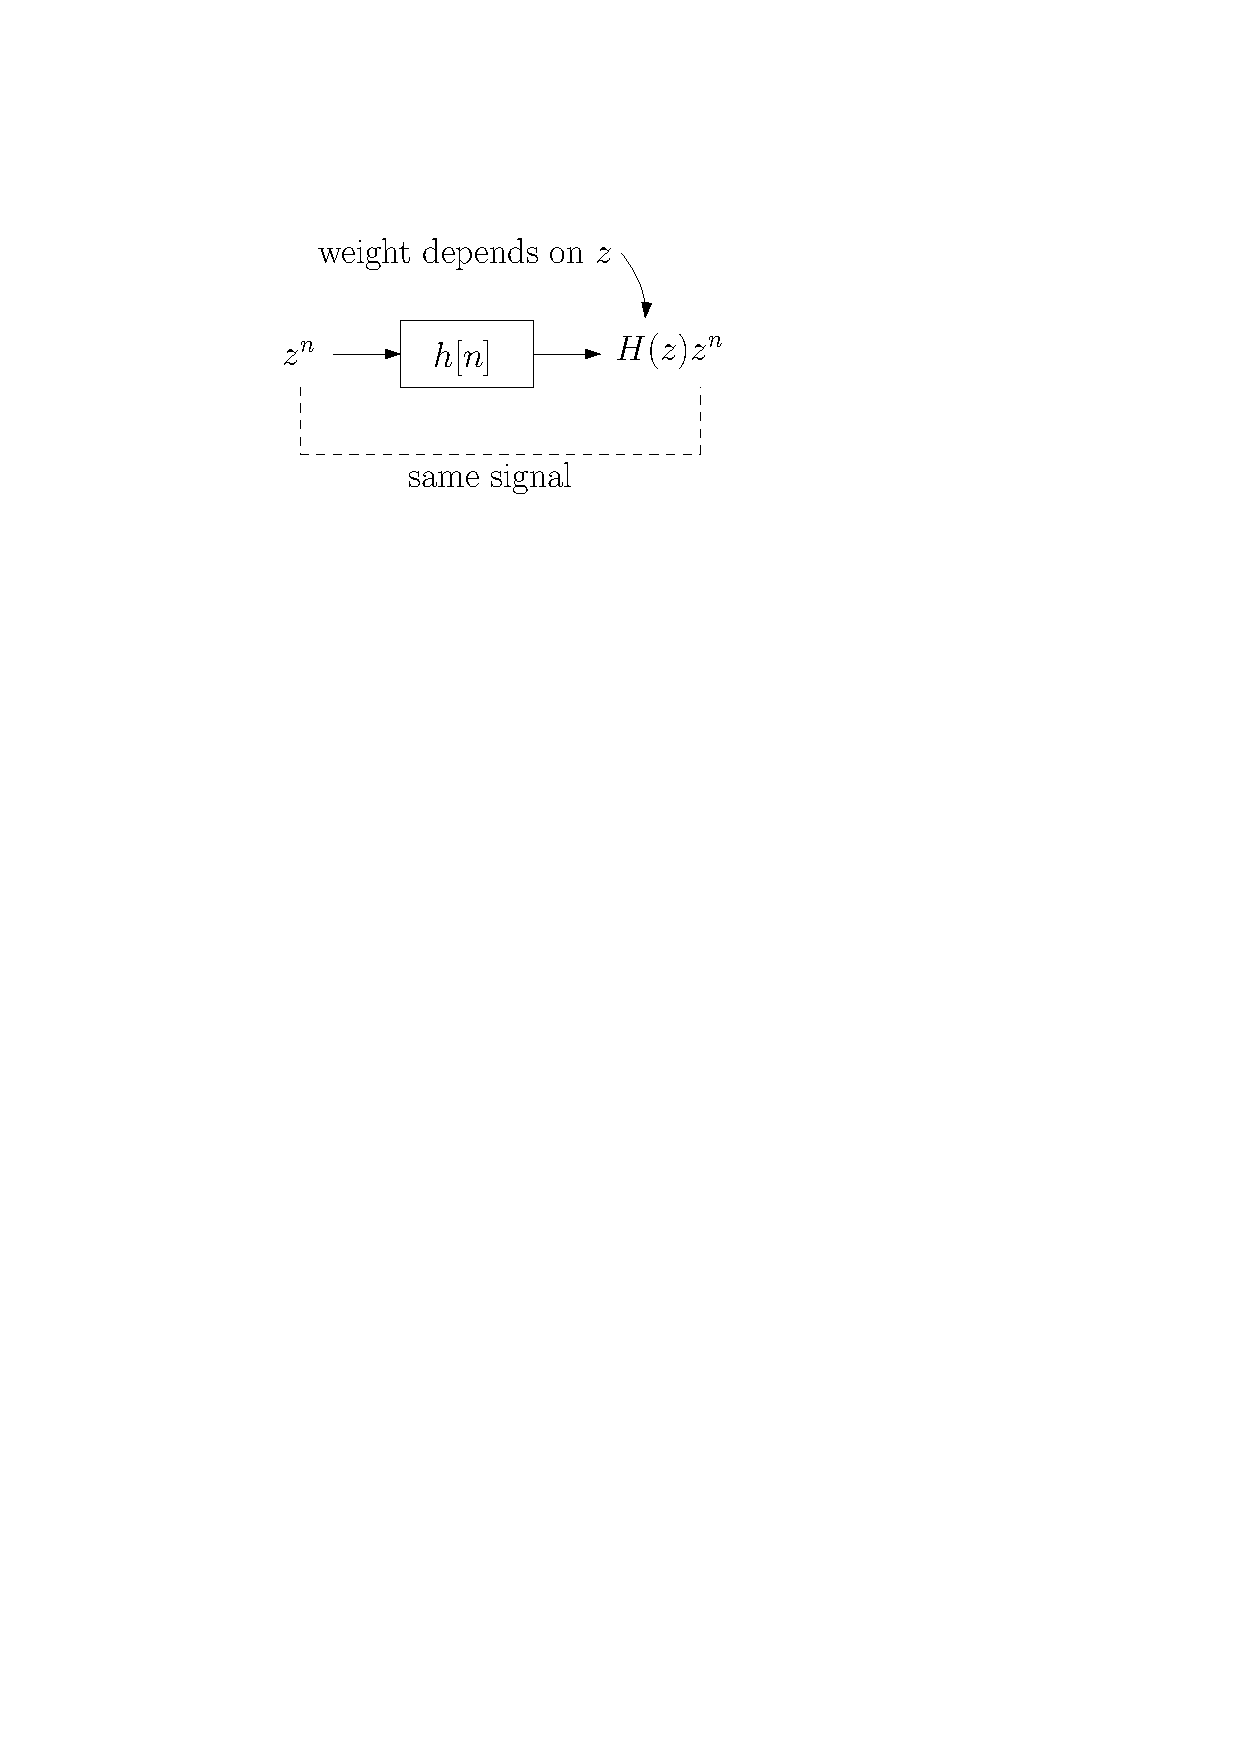
\includegraphics[scale=0.6]{graphics/lti-dt-complex-exp.pdf}
\end{center}

\begin{example}
  For example, suppose $H(z) = \frac{z}{z-\frac{1}{2}}$ and $x[n] = \left(-\frac{1}{4}\right)^n$. Then the output is
  \begin{align*}
    y[n] &= H\left(-\frac{1}{4}\right)\left(-\frac{1}{4}\right)^n\\
    &= \frac{-\frac{1}{4}}{-\frac{1}{4}-\frac{1}{2}}\left(-\frac{1}{4}\right)^n\\
    &= \frac{1}{3}\left(-\frac{1}{4}\right)^n \; ,
  \end{align*}
another complex exponential.\\
$\blacksquare$
\end{example}

Given $H(z)$ and inputs that are sums of complex exponentials, the output is easy to determine.

\begin{center}
  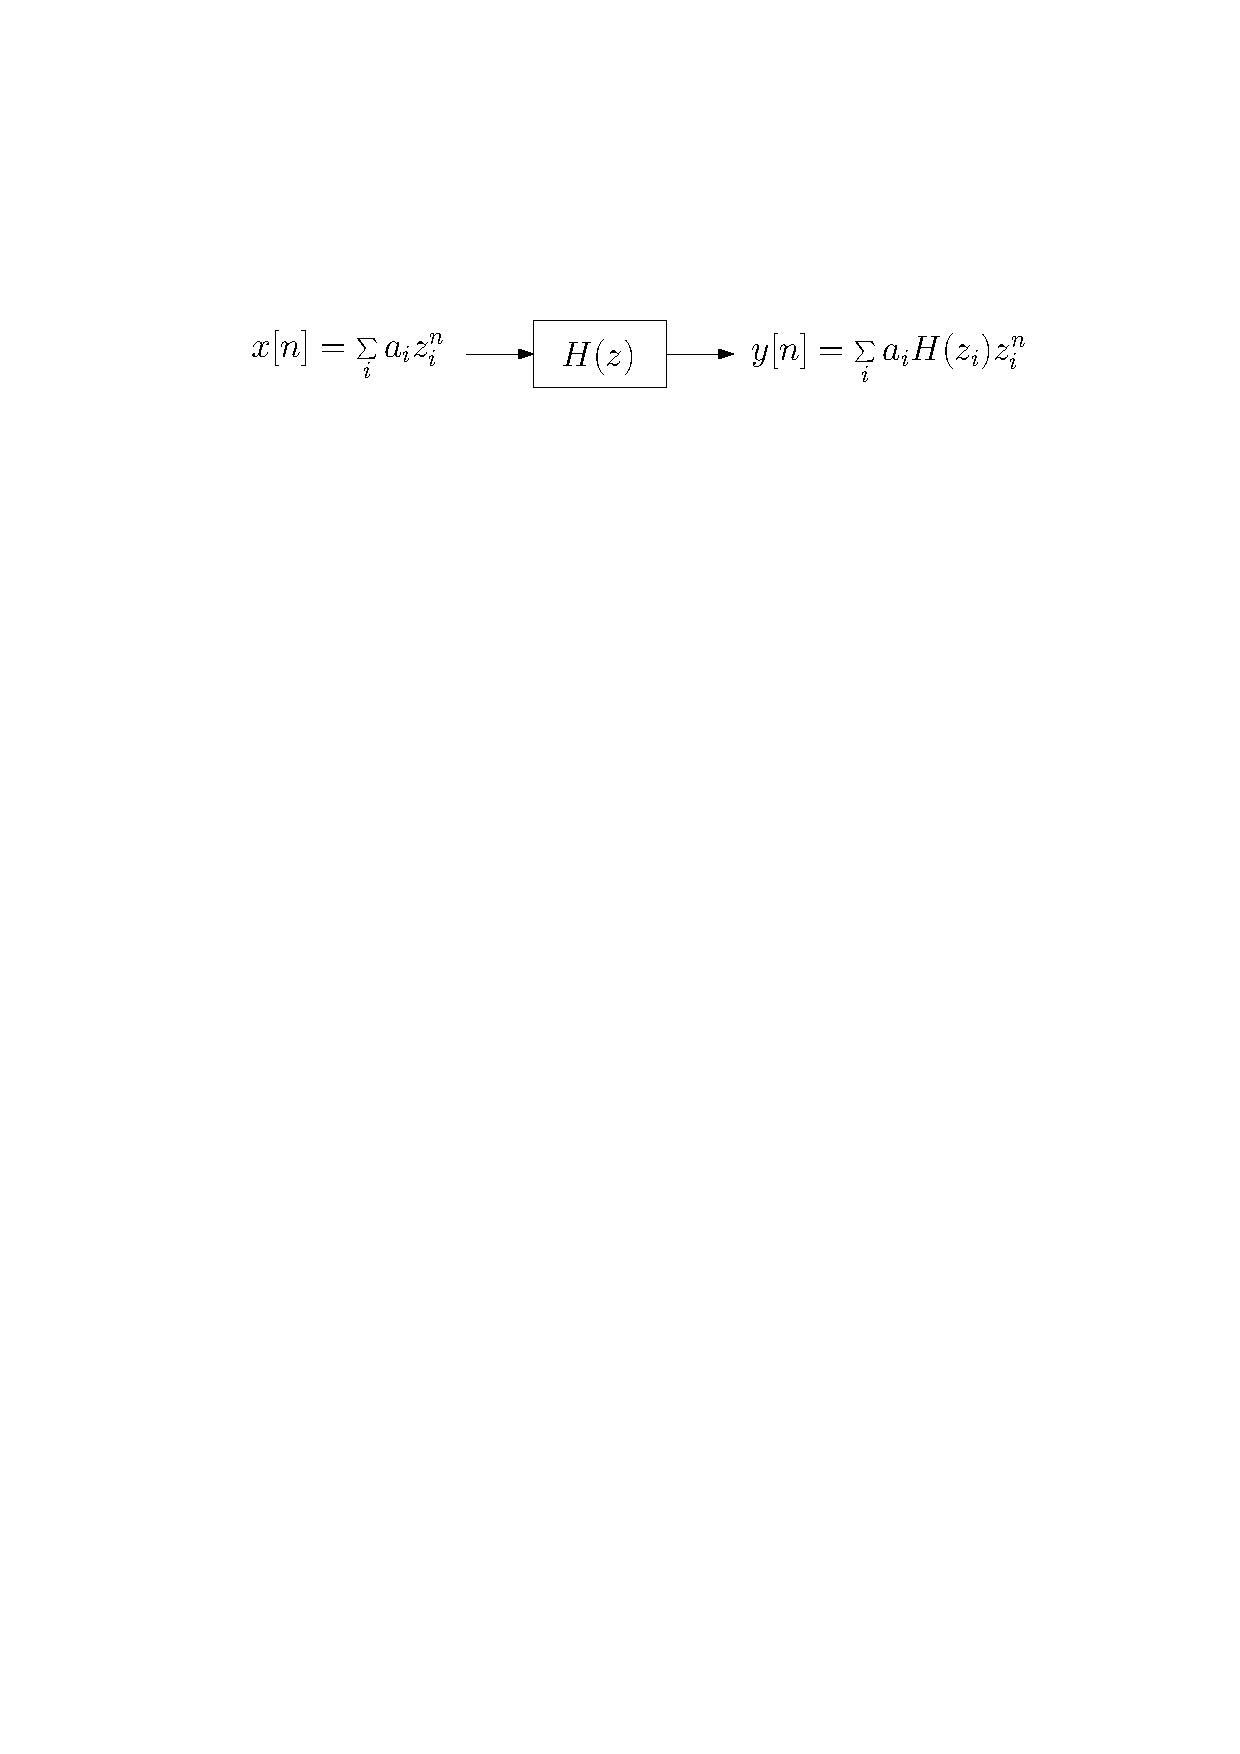
\includegraphics[scale=0.6]{graphics/dt-linear-response-complex-exp.pdf}
\end{center}
In some cases the sums are countably infinite while in others the uncountably infinite so that the sums become integrals.

\begin{example} Consider the DT system with impulse response response
  \[
  h[n] = \left(\frac{3}{4}\right)^{n}u[n]
  \]
  Determine the Eigenvalues that corresponds to the input $x[n] = \cos(n)$ and the output $y[n]$.\\

  Solution: We note the cosine can be decomposed into two complex exponentials as
  \[
  \cos(n) = \frac{1}{2}e^{jn} + \frac{1}{2}e^{-jn} = \frac{1}{2}\left(e^{j}\right)^n + \frac{1}{2}\left(e^{-j}\right)^n
  \]
  Thus in terms of the general decomposition there are two terms with complex constants $z_1 = e^{j}$ and $z_2 = e^{-j}$ and real constants $a_1 = a_2 = \frac{1}{2}$.
  \[
   x[n] = \sum_i a_i z_i^{n} = a_1 z_1^{n} + a_2 z_2^{n} = \frac{1}{2}\left(e^{j}\right)^n + \frac{1}{2}\left(e^{-j}\right)^n = \cos(n)
   \]
   Then the output is given by
   \[
   y[n] = \sum_i H(z_i) a_i z_i^{n} = H(z_1) a_1 z_1^{n} + H(z_2) a_2 z_2^{n} = H\left(e^{j}\right)\frac{1}{2}\left(e^{j}\right)^n + H\left(e^{-j}\right)\frac{1}{2}\left(e^{-j}\right)^n 
   \]
   which requires we find the Eigenvalues $H\left(e^{j}\right)$ and $H\left(e^{-j}\right)$. To do so we use the Z transform summation
   \[
   H\left(e^{j}\right) = \sum\limits_{m = -\infty}^{\infty}h[m]\left(e^{j}\right)^{-m} = \sum\limits_{m = 0}^{\infty} \left(\frac{3}{4}\right)^{m}\left(e^{j}\right)^{-m} = \sum\limits_{m =0}^{\infty} \left(\frac{3}{4\left(e^{j}\right)}\right)^{m} = \frac{-1}{\left(\frac{3}{4e^{j}}\right)-1} = \frac{e^{j}}{e^{j}-\left(\frac{3}{4}\right)}
   \]
   Similarly
   \[
   H\left(e^{-j}\right) = \sum\limits_{m = -\infty}^{\infty}h[m]\left(e^{-j}\right)^{-m} = \sum\limits_{m = 0}^{\infty} \left(\frac{3}{4}\right)^{m}\left(e^{-j}\right)^{-m} = \sum\limits_{m =0}^{\infty} \left(\frac{3}{4\left(e^{-j}\right)}\right)^{m} = \frac{-1}{\left(\frac{3}{4e^{-j}}\right)-1} = \frac{e^{-j}}{e^{-j}-\left(\frac{3}{4}\right)}
   \]

   Substituting back into the output equation gives
   
   \begin{align*}
     y[n] &= H\left(e^{j}\right)\frac{1}{2}\left(e^{j}\right)^n + H\left(e^{-j}\right)\frac{1}{2}\left(e^{-j}\right)^n\\
     &= \frac{e^{j}}{e^{j}-\left(\frac{3}{4}\right)}\frac{1}{2}\left(e^{j}\right)^n + \frac{e^{-j}}{e^{-j}-\left(\frac{3}{4}\right)}\frac{1}{2}\left(e^{-j}\right)^n\\
   \end{align*}
   We can simplify this expression using the polar form of the Eigenvalues
   \begin{align*}
     y[n] &= \frac{e^{j}}{e^{j}-\left(\frac{3}{4}\right)}\frac{1}{2}\left(e^{j}\right)^n + \frac{e^{-j}}{e^{-j}-\left(\frac{3}{4}\right)}\frac{1}{2}\left(e^{-j}\right)^n\\
     &= Re^{j\theta} \frac{1}{2}e^{jn} + Re^{-j\theta} \frac{1}{2}e^{-jn}\\
     &= R \frac{1}{2}e^{jn + j\theta} + R \frac{1}{2}e^{-jn -j\theta}\\
     &= R\cos(n + \theta)
   \end{align*}
   where
   \[
   R = \left|\frac{e^{j}}{e^{j}-\left(\frac{3}{4}\right)}\right| \approx 1.153  \mbox{ and } \theta = \angle{\frac{e^{j}}{e^{j}-\left(\frac{3}{4}\right)}} \approx -0.815
   \]
   Note for this system, given a sinusoidal input, the output is a scaled and phase shifted sinusoid at the same frequency, where the scaling factor and phase shift is system dependent. It is illustrative to compare this analysis to the time-domain analysis of the same impulse response and input using convolution.
   $\blacksquare$
\end{example}

\section{Decomposition of signals using DT complex exponentials}

Similar to CT, in this course we consider the cases of stable DT systems. Recall a stable system is one in which a bounded input leads to a bounded output, or equivalently the impulse response is absolutely summable. We will consider two decompositions of the input:

  \begin{itemize}
  \item \emph{Fourier Series}: When $x[n]$ is periodic with fundamental frequency $\omega_0 = \frac{2\pi}{N}$, $|z| = 1$ so that $z = e^{jk\omega_0}$, and the decomposition is a finite sum. This gives the input-output relationship
    \[
 x[n] = \sum\limits_{k = N_0}^{N_0 + N-1} a_k e^{jk\omega_0n} \;\longrightarrow\;  y[n] = \sum\limits_{k = N_0}^{N_0 + N-1} H\left(e^{j k\omega_0}\right) a_k e^{jk\omega_0 n} 
    \]
    where $H\left(e^{j k\omega_0}\right)$ are the Eigenvalues, also called the DT \emph{frequency response}.
  \item \emph{Inverse Fourier Transform}: When $x[n]$ is a-periodic, $|z| = 1$ so that $z = e^{j\omega}$, and the decomposition is an integral over a finite length set. This gives the input-output relationship
    \[
     x[n] = \frac{1}{2\pi} \int_{2\pi} X\left(e^{j\omega}\right) e^{j\omega n} \; d\omega \;\longrightarrow\;   y[n] = \frac{1}{2\pi} \int_{2\pi} H\left(e^{j\omega}\right) \, X\left(e^{j\omega}\right) e^{j\omega n} \; d\omega
    \]
    where $H\left(e^{j \omega}\right)$ are the Eigenvalues, again called the DT \emph{frequency response}.  
  \end{itemize}

  Other courses such as ECE 3704 look at the general case of unstable systems and $z \in \mathbb{C}$ with decompositions:

  \begin{itemize}
  \item \emph{One-Sided Z Transform}: $x[n]$ is causal and the decomposition is an uncountably infinite sum (complex integral)
  \item \emph{Two-Sided (Bilateral) Z Transform}: $x[n]$ is non-causal and the decomposition is an uncountably infinite sum (complex integral). This is the most general case for DT LTI systems.
  \end{itemize}

  While the Z decompositions require complex integration, like for the Laplace transform in CT, they can be understood and computed using algebra and a table of forward transforms, which only require summations of a complex function over a real variable $n$ (this is the general approach taken in upper level courses). However, this is outside the scope of this course because of time limitations.

Instead, we will be spending the next few weeks going through the DT Fourier decompositions in some detail. You will also learn how to find the DT frequency response for a stable system, and see how to use both for analysis.

